%!TEX spellcheck=ro_RO
%!TEX root = ./main.tex
\chapter{Introducere}\label{ch:1intro}
Ceva despre istoria AI
\section{Temă. Obiective. Motivație}
\textbf{TODO Edit First Paragraph}

Această lucrare are ca scop folosirea Inteligenței Artificiale, mai precis învățarea automată\textit{(machine learning)}, pentru detectarea a trei clase/stării mentale diferite.\ Învățarea automată reprezintă un subdomeniu al Inteligenței Artificiale, fiind folosită la execuția anumitor sarcini fără un mod explicit dat. Tehnicile de învățare automată urmăresc crearea unor modele matematice bazate pe seturi de date inițiale, denumite \textit{seturi de antrenare (training data)}, care pot generaliza informațiile din acestea, iar mai apoi să prezică răspunsul pentru seturi de date necunoscute.

Învățarea automată este folosită intr-o largă gamă de aplicații, precum filtrarea mesajelor e-mail de tip spam de cele autentice, răspunsurile date de către motoarele de căutare, clasificarea celulelor tumorale in benigne sau maligne, recunoașterea facială, recunoașterea diverselor obiecte, recunoașterea limbajului vorbit și scris, și mai nou la conducerea automată a mașinilor. 

Cele mai multe tehnici de învățare automată fac parte din una dintre cele trei categori:
\begin{itemize}
	\item Învățare supervizată (Supervised Learning)
	\item Învățare fără supervizare (Unsupervised Learning)
	\item Învățare cu întărire (Reinforcement Learning)
\end{itemize}

\subsection{Învățarea supervizată}
Învățarea supervizată, în momentul de fața este cea mai răspandită metodă folosită în practică. Principiul din spatele acesteia constând în construirea unui model matematic, prin diferite tehnici, bazat pe un set de date etichetate. Acest set de date etichetate este alcătuit din înregistrări care reprezintă o corespondență intre atribute (intrări) si o clasă (ieșire). Astfel, se urmărește generalizarea acestor corespondețe si posibilitatea prezicerii clasei unei înregistrări care nu aparține de datele folosite la învățare. Unii dintre cei mai folosiți algoritmi de învățare supervizată sunt:
\begin{itemize}
	\item Arbori de decizie
	\item Metode de regresie
	\item Algoritmi genetici
	\item Rețele neuronale artificiale
	\item Mașini cu vector suport
	\item Rețele Bayesiene
\end{itemize}

\subsection{Învățarea nesupervizată}
Procesul de învățare nesupervizată diferă față de cel amintit anterior prin faptul că acesta folosește un set de date de antrenare neetichetat. Algoritmii primesc doar un set de atribute (date de intrare), ne știind ieșirea asociată acestora. Aceștia caută in aceste date asemănări și deosebiri, bazându-se pe proprietățile statistice a datelor. Printre cele mai răspândite tehnici se numără:
\begin{itemize}
	\item Tehnici de grupare
	\subitem Grupare ierarhizată
	\subitem Tehnica k-means
	\item Hărți cu auto-organizare
	\subitem Rețele Kohonen
	\item Modele Markov cu stări invizibile
\end{itemize}

\subsection{Învățarea cu întărire}
Învățarea cu întărire este o metodă de învățare prin interacțiuni repetate, cu urmărirea atingerii unui anumit scop. Un agent \textit{(software agent)} interacţionează pas cu pas prin acţiuni cu mediul înconjurător, acţiunea sa la fiecare pas conducând la modificarea stării acestui mediu (tranziţia la o nouă stare) care îi întoarce ca răspuns (feedback) agentului câte o mărime scalară denumită recompensă (reward). Scopul agentului este maximizarea recompensei cumulate pe termen lung, după o secvenţă de paşi. În acest sens, RL este asemănătoare controlului optimal, utilizând tehnici specifice programării dinamice (procese de decizie Markov) dar fără un model matematic exact al mediului şi funcţionând pe spaţii cu dimensiuni mari \cite{Vrejdoiu:2019}.

\begin{figure}[h]
	\center
	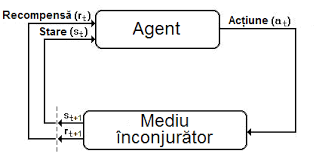
\includegraphics[width=10cm, keepaspectratio]{fig/reinforcement_learning_feedback_loop.png}
	\caption{Modul de interacțiune al agentului cu mediul înconjurător}
\end{figure}


\section{Soluții existente}

\section{Structurare pe capitole}